\section{Differentiation}
\subsection{Basics}

Informally, the derivative of a function is the instantaneous rate of change of a function at that point. \autoref{fig:derivative} shows a way to think about the gradient at some point \(c \in \ccintv{a}{b}\) -- namely approximating the gradient of a secant \(\frac{\delta y}{\delta x}\), and taking the limit as \(h = \delta x \to 0\).

\begin{figure}[ht!]
    \centering
    \begin{tikzpicture}[
        declare function = { f(\x) = 0.6 * (\x - 3) * (\x - 4) * (\x - 5) + 1.5 * (\x - 4) + 7; }
    ]
        \begin{axis}[
            axis lines = middle,
            xlabel = {\(x\)},
            ylabel = {\(f\pqty{x}\)},
            xmin = 0, xmax = 8,
            ymin = 0, ymax = 14,
            samples = 100,
            domain = 2:6,
            xtick = {\xa, \xb, \xc, \xd},
            xticklabels = {\(a\), \(b\), \(c\), \(c + h\)},
            ytick = {\ya, \yb, \yc, \yd},
            yticklabels = {\(f\pqty{a}\), \(f\pqty{b}\), \(f\pqty{c}\), \(f\pqty{c + h}\)}
        ]

            \pgfmathsetmacro{\xa}{2}
            \pgfmathsetmacro{\ya}{f(\xa)}
            \pgfmathsetmacro{\xb}{6}
            \pgfmathsetmacro{\yb}{f(\xb)}
            \pgfmathsetmacro{\xc}{3.5}
            \pgfmathsetmacro{\yc}{f(\xc)}
            \pgfmathsetmacro{\xd}{4.5}
            \pgfmathsetmacro{\yd}{f(\xd)}

            \addplot[no marks] {f(x)};
            \node[right] at (axis cs: 6, 13) {\(f\)};

            \addplot[only marks, mark=*, mark size=1pt]
                coordinates {(\xa, \ya) (\xb, \yb) (\xc, \yc) (\xd, \yd)};

            \addplot[dotted] coordinates {(0, \ya) (\xa, \ya) (\xa, 0)};
            \addplot[dotted] coordinates {(0, \yb) (\xb, \yb) (\xb, 0)};
            \addplot[dotted] coordinates {(0, \yc) (\xc, \yc) (\xc, 0)};
            \addplot[dotted] coordinates {(0, \yd) (\xd, \yd) (\xd, 0)};

            \draw[<->] (axis cs: \xc, \yc) -- (axis cs: \xd, \yc);

            \node[below] at (axis cs: {(\xc + \xd) / 2}, \yc) {\(\delta x\)};

            \draw[<->] (axis cs: \xc, \yc) -- (axis cs: \xc, \yd);

            \node[left] at (axis cs: \xc, {(\yc + \yd) / 2}) {\(\delta y\)};
        \end{axis}
    \end{tikzpicture}

    \caption{Derivative}
    \label{fig:derivative}
\end{figure}

\begin{definition}[Derivative]
    \label{def:derivative}%
    Let \(\functiondomain{f}{X \subseteq \CC}{\CC}\) and \(a \in X\) be an accumulation point. We say \(f\) is \emph{differentiable} at \(a\), if we have
    \[
        \lim_{x \to a} \frac{f\pqty{x} - f\pqty{a}}{x - a} = \lim_{h \to 0} \frac{f\pqty{a + h} - f\pqty{a}}{h}
    \]
    exists. The value of this limit is the \emph{derivative} of \(f\) evaluated at \(a\), denoted as \(f'\pqty{a}\) or \(\dv{f}{x} \pqty{a}\).
\end{definition}

\begin{remark}
    We cannot really make sense of the derivative at an isolated point of the domain, since the point is not in the domain of the fraction, and not an accumulation point of the domain of the fraction either -- so the limit is undefined.

    As for accumulation points, we can distinguish between \emph{interior points}, where we can approach that point along any direction (and we need the limit to be direction independent); and \emph{non-interior points} whose limit is restricted by the domain.
\end{remark}

\begin{examples}[Differentiability of Functions]
    \label{ex:differentiability}%
    \begin{itemize}
        \item We take the identity function \(f\pqty{z} = z\). We have
        \[
            f'\pqty{z} = \lim_{h \to 0} \frac{f\pqty{z + h} - f\pqty{z}}{h} = \lim_{h \to 0} \frac{\pqty{z + h} - z}{h} = \lim_{h \to 0} 1 = 1.
        \]

        \item We take the complex conjugate function \(f\pqty{z} = \conjugate{z}\). We claim this is not differentiable at \emph{any} point.
        
        We consider the limits \(h \to 0\) along the real axis and the complex axis separately.

        Take \(h = \lambda\) for \(\lambda \in \RR\), we have
        \[
            \lim_{\lambda \to 0} \frac{f\pqty{z + \lambda} - f\pqty{z}}{\lambda} = \lim_{\lambda \to 0} \frac{\bar{\lambda}}{\lambda} = \lim_{\lambda \to 0} \frac{\lambda}{\lambda} = 1
        \]
        and \(h = i \lambda\) for \(\lambda \in \RR\), we have
        \[
            \lim_{\lambda \to 0} \frac{f\pqty{z + i \lambda} - f\pqty{z}}{i\lambda} = \lim_{\lambda \to 0} \frac{\conjugate{i \lambda}}{i \lambda} = \lim_{\lambda \to 0} \frac{- i \lambda}{i \lambda} = -1.
        \]

        \item We consider the real sine function \(f\pqty{x} = \sin x\). We have
        \begin{align*}
            f'\pqty{x} &= \lim_{h \to 0} \frac{\sin \pqty{x + h} - \sin \pqty{x}}{h} \\
            &= \lim_{h \to 0} \frac{\sin \pqty{h} \cos x}{h} + \lim_{h \to 0} \frac{\sin x \pqty{\cos h - 1}}{h} \\
            &= \cos x \cdot 1 + 0 \\
            &= \cos x.
        \end{align*}
    \end{itemize}
\end{examples}

Differentiability is a stronger property than continuity -- indeed we cannot differentiate functions that are not continuous.

\begin{proposition}[Differentiability implies Continuity]
    \label{prop:differentiability-implies-continuity}%
    Let \(\functiondomain{f}{X \subseteq \CC}{\CC}\) be differentiable at some \(a \in X\). Then it is continuous at \(a\).
\end{proposition}

\begin{proof}
    Note that
    \begin{align*}
        \bqty{\lim_{h \to 0} f\pqty{x + h}} - f\pqty{x} &= \lim_{h \to 0} \bqty{f\pqty{x + h} - f\pqty{x}} \\
        &= \lim_{h \to 0} \frac{f\pqty{x + h} - f\pqty{x}}{h} \cdot h \\
        &= \lim_{h \to 0} \frac{f\pqty{x + h} - f\pqty{x}}{h} \cdot \lim_{h \to 0} h \\
        &= f'\pqty{x} \cdot 0 \\
        &= 0
    \end{align*}
    gives continuity as desired.
\end{proof}

We may derive properties of derivative from the properties of limits as well.

\begin{lemma}[Properties of Derivatives]
    \label{lem:properties-derivatives}%
    Let \(\functiondomain{f, g}{X \subseteq \CC}{\CC}\) be differentiable at \(a \in X\). Then the sum \(f\pqty{x} + g\pqty{x}\), the product \(f\pqty{x} \cdot g\pqty{x}\), and the reciprocal \(\frac{1}{f\pqty{x}}\) (if defined, i.e. if \(f\pqty{a} \neq 0\)) are all differentiable at \(a\). Furthermore, we have
    \begin{align*}
        \pqty{f + g}' \pqty{a} &= f'\pqty{a} + g'\pqty{a}, \\
        \pqty{fg}' \pqty{a} &= f'\pqty{a} g\pqty{a} + f\pqty{a} g'\pqty{a}, \\
        \pqty{\frac{1}{f}}' \pqty{a} &= - \frac{f'\pqty{a}}{\bqty{f\pqty{a}}^2}.
    \end{align*}
\end{lemma}

\begin{proof}
    The addition rule is trivial from \autoref{lem:fn-limits-preserve-arithmetic}.

    We now look at the product.
    \begin{align*}
        \pqty{fg}'\pqty{a} &= \lim_{h \to 0} \frac{\pqty{fg}\pqty{a + h} - \pqty{fg}\pqty{a}}{h} \\
        &= \lim_{h \to 0} \frac{f\pqty{a + h} g\pqty{a + h} - f\pqty{a} g\pqty{a}}{h} \\
        &= \lim_{h \to 0} \frac{\pqty{f\pqty{a + h} - f\pqty{a}} g\pqty{a + h} + \pqty{g\pqty{a + h} - g\pqty{a}} f\pqty{a}}{h} \\
        &= \lim_{h \to 0} g\pqty{a + h} \cdot \lim_{h \to 0} \frac{f\pqty{a + h} - f\pqty{a}}{h} + f\pqty{a} \cdot \lim_{h \to 0} \frac{g\pqty{a + h} - g\pqty{a}}{h} \\
        &= g\pqty{a} \cdot f'\pqty{a} + f\pqty{a} \cdot g'\pqty{a},
    \end{align*}
    using continuity (implied by differentiability, stated in \autoref{prop:differentiability-implies-continuity}), in \(\lim_{h \to 0} g\pqty{a + h} = g\pqty{a}\).

    As for the reciprocal,
    \begin{align*}
        \pqty{\frac{1}{f}}'\pqty{a} &= \lim_{h \to 0} \frac{\frac{1}{f\pqty{a + h}} - \frac{1}{f\pqty{a}}}{h} \\
        &= \lim_{h \to 0} \frac{f\pqty{a} - f\pqty{a + h}}{h} \cdot \frac{1}{f\pqty{a} f\pqty{a + h}} \\
        &= - \lim_{h \to 0} \frac{1}{f\pqty{a} f\pqty{a + h}} \cdot \lim_{h \to 0} \frac{f\pqty{a + h} - f\pqty{a}}{h} \\
        &= - \frac{f'\pqty{a}}{\bqty{f\pqty{a}}^2}.
    \end{align*}
\end{proof}

\begin{examples}[Applications of Differentiation Rules]
    \label{ex:aplication-of-differentiation-rules}%
    \begin{itemize}
        \item Let \(f\pqty{z} = z^2\), then it is differentiable with \(f'\pqty{z} = 2z\). By induction, for \(f\pqty{z} = z^n\) with \(n \in \NN\), we have \(f'\pqty{z} = n z^{n - 1}\).
        \item Let \(f\pqty{z} = \frac{1}{z}\). It is differentiable on \(\CC \setminus\Bqty{0}\) with \(f'\pqty{z} = -\frac{1}{z^2}\). By induction, for \(f\pqty{z} = \frac{1}{z^n}\), we have \(f'\pqty{z} = - \frac{n}{z^{n + 1}}\).
        \item More generally, rational functions \(\frac{p\pqty{x}}{q\pqty{x}}\) for polynomials \(p, q\) are differentiable, wherever it is defined.
    \end{itemize}
\end{examples}

\begin{proposition}[Chain Rule]
    \label{prop:chain-rule}%
    Let \(U, V \subseteq \CC\), and let \(\functiondomain{f}{U}{V}\), and \(\functiondomain{g}{V}{\CC}\). Suppose \(f\) is differentiable at some \(a \in U\), and \(g\) is differentiable at some \(f\pqty{a} \in V\). Then the composition \(g \circ f\) is differentiable at \(a\), and that
    \[
        \pqty{g \circ f}'\pqty{a} = g' \pqty{f\pqty{a}} \cdot f'\pqty{a}.
    \]
\end{proposition}

\begin{proof}
    One might be very tempted to say that
    \[
        \frac{g\pqty{f\pqty{x}} - g\pqty{f\pqty{a}}}{x - a} = \frac{g\pqty{f\pqty{x}} - g\pqty{f\pqty{a}}}{f\pqty{x} - f\pqty{a}} \cdot \frac{f\pqty{x} - f\pqty{a}}{x - a}
    \]
    and this finishes the proof. However, we need to deal with the case where we are dividing by zero. Therefore, we define a helper function
    \[
        Q\pqty{y} = \begin{cases}
            \frac{g\pqty{y} - g\pqty{f\pqty{a}}}{y - f\pqty{a}}, & y \neq f\pqty{a}, \\
            g'\pqty{f\pqty{a}}, & y = f\pqty{a},
        \end{cases}
    \]
    and we claim that the quotient is always equal to
    \[
        Q\pqty{f\pqty{x}} \cdot \frac{f\pqty{x} - f\pqty{a}}{x - a}.
    \]

    For any \(x \neq a\), if \(f\pqty{x} \neq f\pqty{a}\), then the equality is from the cancellation of fraction from above. If \(x \neq a\) but \(f\pqty{x} = f\pqty{a}\), then the quotient is zero, and this expression is zero as well since the second term is zero.

    Now it remains to take the limit of this expression. As \(x \to a\), the second factor tends to \(f'\pqty{a}\). For \(Q\pqty{y}\), note that since \(g\) is differentiable at \(f\pqty{a}\), so we have
    \[
        \lim_{y \to f\pqty{a}} Q\pqty{y} = g'\pqty{f\pqty{a}} = Q\pqty{f\pqty{a}}
    \]
    so \(Q\) is continuous at \(f\pqty{a}\). Furthermore, \(f\) is differentiable at \(a\), and hence continuous. Therefore, \(Q \circ f\) is continuous at \(a\), so its limit is simply \(Q\circ f\pqty{a} = g'\pqty{f\pqty{a}}\).

    Taking the product of the limit of the two factors, we have
    \[
        g \circ f'\pqty{a} = g'\pqty{f\pqty{a}} \cdot f'\pqty{a}
    \]
    as desired.
\end{proof}

We may provide another characterisation of the derivative to give a proof of \autoref{prop:chain-rule} (Chain Rule) which could be generalised to higher dimensions.

We have seen that \(f'\pqty{a}\) is the slope of the tangent line to the graph of \(f\) at \(a\). We can formalise this in the following way.

\begin{lemma}[Linear Approximation and Differentiability]
    \label{lem:linear-approximation-differentiability}%
    Let \(\functiondomain{f}{X \subseteq \CC}{\CC}\). Then \(f\) be differentiable at \(a\), if and only if there is some \(A \in \CC\), and a function \(\functiondomain{\epsilon}{\set{z \in \CC}{z + a \in X}}{\CC}\) (an error function), with \(\epsilon\pqty{h} \to 0\) as \(h \to 0\), such that
    \[
        f\pqty{a + h} = f\pqty{a} + A h + \epsilon\pqty{h} \abs{h}.
    \]

    In particular, such \(A\) is \(f'\pqty{a}\).
\end{lemma}

\begin{remark}
    This says that \(f\pqty{a + h}\) is approximately \(f\pqty{x} + Ah\), and the error function \(\epsilon\pqty{h}\) is to quantify the error in this approximation. This is also much easier to generalise to higher dimensions for functions in more general spaces (Banach spaces). In this more general case, \(A\) will be a linear operator.
\end{remark}

We can also write that \(f\pqty{a + h} = f\pqty{a} + Ah + \littleO\pqty{h}\) using the little-\(\littleO\) notation (and not big-\(\bigO\)) to mean the same thing.

\begin{proof}[of \autoref{lem:linear-approximation-differentiability}]
    We assume there is such linear approximation. Then
    \begin{align*}
        \lim_{h \to 0} \frac{f\pqty{a + h} - f\pqty{a}}{h} &= \lim_{h \to 0} \frac{Ah + \epsilon\pqty{h} \cdot \abs{h}}{h} \\
        &= A + \lim_{h \to 0} \pqty{\epsilon\pqty{h} \cdot \frac{\abs{h}}{h}} \\
        &= A + 0 \\
        &= A,
    \end{align*}
    since \(\frac{\abs{h}}{h}\) is bounded and \(\epsilon\pqty{h} \to 0\). Therefore, \(f\) is differentiable at \(a\), and hence \(f'\pqty{a} = A\).

    On the other hand, if the function is differentiable at \(a\), let \(A = f'\pqty{a}\). We take the error function
    \[
        \epsilon\pqty{h} = \begin{cases}
            \frac{f\pqty{a + h} - f\pqty{a} - Ah}{\abs{h}}, & h \neq 0, \\
            0, & h = 0.
        \end{cases}
    \]
    Then we can see by taking limits that \(\epsilon\pqty{h} \to 0\) as \(h \to 0\).
\end{proof}

\begin{proof}[of \autoref{prop:chain-rule} (Chain Rule)]
    Since \(f, g\) are differentiable at \(a, f\pqty{a}\) respectively, there exist some error functions \(\epsilon_f, \epsilon_g\) such that \(\epsilon_f\pqty{h}, \epsilon_g\pqty{h} \to 0\) as \(h \to 0\), and that
    \[
        f\pqty{a + h} = f\pqty{a} + f'\pqty{a} h + \epsilon_f\pqty{h} \abs{h}
    \]
    and similarly
    \[
        g\pqty{f\pqty{a} + k} = g\pqty{f\pqty{a}} + g'\pqty{f\pqty{a}} k + \epsilon_g\pqty{k} \abs{k}.
    \]

    We now investigate the composition. Note that
    \begin{align*}
        g \circ f\pqty{a + h} - g \circ f\pqty{a} &= g\pqty{f\pqty{a + h}} - g\pqty{f\pqty{a}} \\
        &= g\pqty{f\pqty{a} + f'\pqty{a} h + \epsilon_f\pqty{h} \abs{h}} - g\pqty{f\pqty{a}} \\
        &= g\pqty{f\pqty{a}} + g'\pqty{f\pqty{a}} \cdot k + \epsilon_g \pqty{k} \cdot \abs{k} - g\pqty{f\pqty{a}} \\
        &= g'\pqty{f\pqty{a}} \cdot k + \epsilon_g\pqty{k} \abs{k}
    \end{align*}
    where we let
    \[
        k = f'\pqty{a}h + \epsilon_f\pqty{h} \abs{h}.
    \]

    Hence,
    \begin{align*}
        g \circ f\pqty{a + h} - g \circ f\pqty{a} &= g'\pqty{f\pqty{a}} f'\pqty{a} h + g'\pqty{f\pqty{a}} \epsilon_f\pqty{h} \abs{h} + \epsilon_g\pqty{k} \abs{k} \\
        &= g'\pqty{f\pqty{a}} f'\pqty{a} h + \epsilon\pqty{h} \abs{h}
    \end{align*}
    where we let
    \[
        \epsilon\pqty{h} = g'\pqty{f\pqty{a}} \epsilon_f\pqty{h} + \epsilon_g\pqty{h f'\pqty{a} + \epsilon_f\pqty{h} \abs{h}} \cdot \abs{\pm f'\pqty{a} + \epsilon_f\pqty{h}},
    \]
    where the \(\pm\) sign arises since we extracted \(h\) with \(\abs{h}\) out from the absolute value of \(k\).

    We want to check that \(\epsilon\pqty{h} \to 0\) as \(h \to 0\). We conduct the limit term-by-term. Note that indeed,
    \[
        \lim_{h \to 0} \bqty{g'\pqty{f\pqty{a}} \epsilon_f\pqty{h}} = g'\pqty{f\pqty{a}} \lim_{h \to 0} \epsilon_f\pqty{h} = 0,
    \]
    and since the inside term of the function \(\epsilon_g\) satisfies
    \[
        \lim_{h \to 0} \bqty{h f'\pqty{a} + \epsilon_f\pqty{h} \abs{h}} = 0
    \]
    and also
    \[
        \lim_{h \to 0} \abs{\pm f'\pqty{a} + \epsilon_f\pqty{h}} = \abs{f'\pqty{a}},
    \]
    we have \(\epsilon\pqty{h} \to 0\). This proves the chain rule indeed.
\end{proof}

\begin{example}[Application of the Chain Rule]
    \label{ex:application-chain-rule}%
    We let
    \[
        f\pqty{x} = \begin{cases}
            x \sin \pqty{\frac{1}{x}}, & x \neq 0, \\
            0, & x = 0.
        \end{cases}
    \]

    At \(x \neq 0\), the chain rule gives us that
    \[
        f'\pqty{x} = 1 \cdot \sin \pqty{\frac{1}{x}} + x \cdot \cos \pqty{\frac{1}{x}} \cdot \pqty{- \frac{1}{x^2}} = \sin \pqty{\frac{1}{x}} - \frac{1}{x} \cos \pqty{\frac{1}{x}}.
    \]

    At \(x = 0\), we have
    \[
        f'\pqty{0} = \lim_{h \to 0} \frac{f\pqty{h} - f\pqty{0}}{h} = \lim_{h \to 0} \sin \pqty{\frac{1}{h}}
    \]
    does not exist. Hence, \(f\) is not differentiable at \(0\). \(f\) is differentiable on \(\RR \setminus \Bqty{0}\).
\end{example}

\autoref{lem:linear-approximation-differentiability} gives another way to prove \autoref{prop:differentiability-implies-continuity} (Differentiability implies Continuity).

\begin{proof}[of \autoref{prop:differentiability-implies-continuity}]
    Recall that we have
    \begin{align*}
        f\pqty{x} &= \lim_{h \to 0} f\pqty{a + h} \\
        &= \lim_{h \to 0} \pqty{f\pqty{a} + Ah + \epsilon\pqty{h} \cdot \abs{h}} \\
        &= f\pqty{a} + A \cdot \lim_{h \to 0} h + \lim_{h \to 0} \cdot \pqty{\epsilon\pqty{h} \cdot \abs{h}} \\
        &= f\pqty{a}.
    \end{align*}
\end{proof}

\subsection{Mean Value Theorems}

\begin{theorem}[Mean Value Theorem]
    \label{thm:mean-value-thm}%
    Let \(\functiondomain{f}{\ccintv{a}{b}}{\RR}\) be continuous on \(\ccintv{a}{b}\) and differentiable on \(\oointv{a}{b}\). Then there is some \(c \in \oointv{a}{b}\) such that
    \[
        f'\pqty{c} = \frac{f\pqty{b} - f\pqty{a}}{b - a}.
    \]
\end{theorem}

\begin{figure}[ht!]
    \centering
    \begin{tikzpicture}[
        declare function = { f(\x) = 0.3 * (\x - 1) * (\x - 3) * (\x - 5) + 3 + (\x - 3); }
    ]
        \begin{axis}[
            axis lines = middle,
            xlabel = {\(x\)},
            ylabel = {\(y\)},
            xmin = -0.5, xmax = 6.5,
            ymin = -0.5, ymax = 6.5,
            samples = 200,
            domain = \xa:\xb,
            xtick = {\xa, \xb},
            xticklabels = {\(a\), \(b\)},
            ytick = {\ya, \yb},
            yticklabels = {\(f\pqty{a}\), \(f\pqty{b}\)},
            width = 12cm
        ]
            \pgfmathsetmacro{\xa}{1}
            \pgfmathsetmacro{\xb}{5}
            \pgfmathsetmacro{\ya}{f(\xa)}
            \pgfmathsetmacro{\yb}{f(\xb)}

            \pgfmathsetmacro{\xc}{3 - 2 * sqrt(3) / 3}
            \pgfmathsetmacro{\xd}{3 + 2 * sqrt(3) / 3}
            \pgfmathsetmacro{\yc}{f(\xc)}
            \pgfmathsetmacro{\yd}{f(\xd)}

            \pgfmathsetmacro{\m}{(\yb - \ya) / (\xb - \xa)}

            \addplot[no marks] {f(x)};

            \addplot[densely dashed, domain=0.5:5.5] {\ya + \m * (x - \xa)};

            \addplot[only marks, mark=*, mark size=1pt]
            coordinates {(\xa, \ya) (\xb, \yb) (\xc, \yc) (\xd, \yd)};

            \addplot[dashed, domain=1:3] {\yc + \m * (x - \xc)};
            \addplot[dashed, domain=3:5] {\yd + \m * (x - \xd)};
            
            \node[above left] at (axis cs: \xc, \yc) {\(f'\pqty{c_1} = \frac{f\pqty{b} - f\pqty{a}}{b - a}\)};
            \node[below right] at (axis cs: \xd, \yd) {\(f'\pqty{c_2} = \frac{f\pqty{b} - f\pqty{a}}{b - a}\)};
            \node[below right] at (axis cs: \xa, \ya) {\(\pqty{a, f\pqty{a}}\)};
            \node[above left] at (axis cs: \xb, \yb) {\(\pqty{b, f\pqty{b}}\)};
        \end{axis}
    \end{tikzpicture}

    \caption{Mean Value Theorem}
    \label{fig:mean-value}
\end{figure}

We introduce \autoref{thm:rolle} (which is a special case of \autoref{thm:mean-value-thm} (Mean Value Theorem)), whose proof is slightly easier -- but this can in fact be used to prove \autoref{thm:mean-value-thm} (Mean Value Theorem).

\begin{theorem}[Rolle's Theorem]
    \label{thm:rolle}%
    Let \(\functiondomain{f}{\ccintv{a}{b}}{\RR}\) be continuous on \(\ccintv{a}{b}\) and differentiable on \(\oointv{a}{b}\). If \(f\pqty{a} = f\pqty{b}\), then there is some \(c \in \oointv{a}{b}\) such that
    \[
        f'\pqty{c} = 0.
    \]
\end{theorem}

\begin{figure}[ht!]
    \centering
    \begin{tikzpicture}[
        declare function = { f(\x) = 0.3 * (\x - 1) * (\x - 3) * (\x - 5) + 3; }
    ]
        \begin{axis}[
            axis lines = middle,
            xlabel = {\(x\)},
            ylabel = {\(y\)},
            xmin = -0.5, xmax = 6.5,
            ymin = 1.5, ymax = 4.5,
            samples = 200,
            domain = \xa:\xb,
            xtick = {\xa, \xb},
            xticklabels = {\(a\), \(b\)},
            ytick = {\ya},
            yticklabels = {\(f\pqty{a} = f\pqty{b}\)},
            width = 12cm
        ]
            \pgfmathsetmacro{\xa}{1}
            \pgfmathsetmacro{\xb}{5}
            \pgfmathsetmacro{\ya}{f(\xa)}
            \pgfmathsetmacro{\yb}{f(\xb)}

            \pgfmathsetmacro{\xc}{3 - 2 * sqrt(3) / 3}
            \pgfmathsetmacro{\xd}{3 + 2 * sqrt(3) / 3}
            \pgfmathsetmacro{\yc}{f(\xc)}
            \pgfmathsetmacro{\yd}{f(\xd)}

            \pgfmathsetmacro{\m}{(\yb - \ya) / (\xb - \xa)}

            \addplot[no marks] {f(x)};

            \addplot[densely dashed, domain=0.5:5.5] {\ya + \m * (x - \xa)};

            \addplot[only marks, mark=*, mark size=1pt]
            coordinates {(\xa, \ya) (\xb, \yb) (\xc, \yc) (\xd, \yd)};

            \addplot[dashed, domain=1:3] {\yc + \m * (x - \xc)};
            \addplot[dashed, domain=3:5] {\yd + \m * (x - \xd)};
            
            \node[above] at (axis cs: \xc, \yc) {\(f'\pqty{c_1} = 0\)};
            \node[below] at (axis cs: \xd, \yd) {\(f'\pqty{c_2} = 0\)};
            \node[below] at (axis cs: \xa, \ya) {\(\pqty{a, f\pqty{a}}\)};
            \node[above] at (axis cs: \xb, \yb) {\(\pqty{b, f\pqty{b}}\)};
        \end{axis}
    \end{tikzpicture}

    \caption{Rolle's Theorem}
    \label{fig:rolle}
\end{figure}

\autoref{fig:mean-value} shows an illustration for \autoref{thm:mean-value-thm} (Mean Value Theorem), while \autoref{fig:rolle} gives an illustration for \autoref{thm:rolle} (Rolle's Theorem). Indeed, they are related by simply adding/subtracting a linear function (which has gradient equal to the secant), as would be illustrated in the proof below.

\begin{proof}[of \autoref{thm:mean-value-thm} (Mean Value Theorem) using \autoref{thm:rolle} (Rolle's Theorem)]
    We define a new function
    \[
        l\pqty{x} = \frac{f\pqty{b} - f\pqty{a}}{b - a} \cdot \pqty{x - a} + f\pqty{a},
    \]
    and let
    \[
        \phi\pqty{x} = f\pqty{x} - l\pqty{x}.
    \]

    Then \(\phi\pqty{a} = \phi\pqty{b} = 0\), and \(\phi'\pqty{x} = f'\pqty{x} - \frac{f\pqty{b} - f\pqty{a}}{b - a}\). Note that since \(f\) is continuous on \(\ccintv{a}{b}\) and differentiable on \(\oointv{a}{b}\), so is \(\phi\), and hence by \autoref{thm:rolle} (Rolle's Theorem) there is some \(c \in \oointv{a}{b}\), such that
    \[
        \phi'\pqty{c} = 0.
    \]

    At \(x = c\), we have
    \[
        f'\pqty{c} = \phi'\pqty{c} + l'\pqty{c} = \frac{f\pqty{b} - f\pqty{a}}{b - a},
    \]
    as desired.
\end{proof}

\begin{remark}
    A corollary of \autoref{thm:mean-value-thm} (Mean Value Theorem) is as follows: given \(h\) such that \(a + h \in \ccintv{a}{b}\), we have some \(\theta = \theta\pqty{h} \in \oointv{0}{1}\), such that
    \[
        f\pqty{a + h} + f\pqty{a} + h f'\pqty{a + h \theta \pqty{h}}.
    \]

    Notice the similarity of \autoref{lem:linear-approximation-differentiability} -- but here we have no error term, but the derivative is taken at some other point.
\end{remark}

We now look back at \autoref{thm:rolle} (Rolle's Theorem).

\begin{proof}[of \autoref{thm:rolle} (Rolle's Theorem)]
    By \autoref{thm:extreme-value} (Extreme Value Theorem), \(f\) attains its maximum and minimum values on \(\ccintv{a}{b}\), i.e., there are \(x_m, x_M \in \ccintv{a}{b}\), such that
    \[
        \sup_{x \in \ccintv{a}{b}} f = f\pqty{x_M} \qand \inf_{x \in \ccintv{a}{b}} f = f\pqty{x_m}.
    \]

    If \(x_m \in \oointv{a}{b}\), we have
    \[
        \sign \pqty{\frac{f\pqty{x_m + h} - f\pqty{x_m}}{{h}}} = \sign \pqty{h}.
    \]

    Hence, by taking \(h_n \to 0^-\) and \(h_n \to 0^+\), we see \(f'\pqty{x_m} = 0\).

    Similarly, if \(x_M \in \oointv{a}{b}\), then
    \[
        \sign \pqty{\frac{f\pqty{x_M + h} - f\pqty{x_M}}{h}} = - \sign\pqty{h}
    \]
    and similarly as before, we have \(f'\pqty{x_M} = 0\).

    If both the maximum and the minimum are attained at endpoints, this means the function is constant, and therefore the result is trivially true.
\end{proof}

\begin{corollary}[Sign of Derivative and Monotonicity]
    \label{cor:sign-of-derivative-monotonicity}%
    Let \(\functiondomain{f}{\ccintv{a}{b}}{\RR}\) be continuous on \(\ccintv{a}{b}\) and differentiable on \(\oointv{a}{b}\). Then
    \begin{itemize}
        \item if \(f'\pqty{x} \geq 0\) on \(\oointv{a}{b}\), then \(f\) is increasing;
        \item if \(f'\pqty{x} > 0\) on \(\oointv{a}{b}\), then \(f\) is strictly increasing;
        \item if \(f'\pqty{x} \leq 0\) on \(\oointv{a}{b}\), then \(f\) is decreasing;
        \item if \(f'\pqty{x} < 0\) on \(\oointv{a}{b}\), then \(f\) is strictly decreasing;
        \item if \(f'\pqty{x} = 0\) on \(\oointv{a}{b}\), then \(f\) is constant.
    \end{itemize}
\end{corollary}

\begin{proof}
    The final case is just a straightforward application of the first and the third case. The third and fourth case are equivalent to the first two.

    We show it for the first case, and the proof can be adapted to the second case easily by removing/adding equal signs.

    Suppose for the sake of contradiction that \(f\) is not increasing. Then for some \(a \leq c < d \leq d\) we have \(f\pqty{c} > f\pqty{d}\). By \autoref{thm:mean-value-thm} (Mean Value Theorem), there is some \(\xi \in \oointv{c}{d}\) such that
    \[
        f'\pqty{\xi} = \frac{f\pqty{c} - f\pqty{d}}{c - d} < 0
    \]
    which contradicts with \(f'\pqty{\xi} \geq 0\). This then finishes the proof.
\end{proof}

\begin{remark}
    We cannot always replace \(\ccintv{a}{b}\) with some set \(X \subseteq \RR\). For instance, the function
    \[
        \function{f}{\QQ}{\RR}{x}{\begin{cases}
            0, & x^2 > 2, \\
            1, & x^2 < 2.
        \end{cases}}
    \]

    This is continuous at any point in its domain, so it is continuous, and \(f'\pqty{x} = 0\) for any \(x \in \QQ\). However, this function is not constant.
\end{remark}

\begin{lemma}[Zero Derivative implies Constant]
    \label{lem:zero-derivative-constant}%
    For a differentiable function \(\functiondomain{f}{\CC}{\CC}\), and that \(f'\pqty{z} = 0\) for all \(z \in \CC\), then \(f\) is constant.
\end{lemma}

\begin{proof}
    Our strategy is to reduce this to the \(\RR\) case. We fix some \(z \in \CC\) with \(z \neq 0\). We take
    \[
        g\pqty{t} = f\pqty{tz}
    \]
    where \(\functiondomain{g}{\ccintv{0}{1}}{\CC}\). Note that \(g\) is continuous on \(\ccintv{0}{1}\), and \(g\) is differentiable on \(\oointv{0}{1}\). We have
    \[
        g'\pqty{t} = z f'\pqty{tz} = 0
    \]
    for all \(z \in \CC\). Furthermore, we have
    \[
        g\pqty{t} = \Re\pqty{g} \pqty{t} + i \cdot \Im\pqty{g} \pqty{t}
    \]
    and hence
    \[
        g'\pqty{t} = \pqty{\Re \pqty{g}}' \pqty{t} + i \pqty{\Im \pqty{g}}' \pqty{t} = 0.
    \]
    
    So \(\pqty{\Re\pqty{g}}' \pqty{t} = \pqty{\Im \pqty{g}}' \pqty{t} = 0\). Applying \autoref{cor:sign-of-derivative-monotonicity} to \(\Re\pqty{g}\) and \(\Im\pqty{g}\), we have both of them are constant, so \(g\) is constant. In particular, \(g\pqty{0} = g\pqty{1} = f\pqty{z}\).

    But \(z\) was arbitrary, so \(f\pqty{z} = f\pqty{0}\) for all \(z \in \CC\).
\end{proof}

\begin{theorem}[Inverse Function Theorem for Differentiability]
    \label{thm:inverse-fn-thm-differentiable}%
    Let \(\functiondomain{f}{\ccintv{a}{b}}{\RR}\) be continuous on \(\ccintv{a}{b}\) and differentiable on \(\oointv{a}{b}\), with \(f'\pqty{x} > 0\) for all \(x \in \oointv{a}{b}\). Then \(\functiondomain{f}{\ccintv{a}{b}}{\ccintv{f\pqty{a}}{f\pqty{b}}}\) is bijective, with its inverse \(\functiondomain{f\inverse}{\ccintv{f\pqty{a}}{f\pqty{b}}}{\ccintv{a}{b}}\) being continuous and differentiable in \(\oointv{f\pqty{a}}{f\pqty{b}}\) with
    \[
        \pqty{f\inverse}' \pqty{y} = \frac{1}{f'\pqty{f\inverse\pqty{y}}}.
    \] 
\end{theorem}

\begin{proof}
    By \autoref{cor:sign-of-derivative-monotonicity}, \(f\) is strictly increasing, and by \autoref{thm:inverse-fn-thm-monotone}, \(f\) is bijection and \(f\inverse\) is continuous. It remains to show the differentiability part.

    Let \(y \in \oointv{f\pqty{a}}{f\pqty{b}}\), and let \(x = f\inverse\pqty{y}\) be its unique pre-image. Given \(h\) such that \(y + h \in \oointv{f\pqty{a}}{f\pqty{b}}\), we take \(k\) such that \(y + h = f\pqty{x + k}\). In other words, let
    \[
        k = f\inverse\pqty{y + h} - x.
    \]

    Then, we have
    \begin{align*}
        \frac{f\inverse\pqty{y + h} - f\inverse\pqty{y}}{h} &= \frac{\pqty{x + k} - x}{f\pqty{x + k} - y} \\
        &= \frac{k}{f\pqty{x + k} - f\pqty{x}} \\
        &= \frac{1}{\frac{f\pqty{x + k} - f\pqty{x}}{k}}.
    \end{align*}

    As \(h \to 0\), the left-hand side has a limit of \(\pqty{f\inverse}' \pqty{y}\) by definition. Furthermore, we have
    \[
        \lim_{h \to 0} k = \pqty{\lim_{h \to 0} f\inverse\pqty{y + h}} - x = f\inverse\pqty{y} - x = 0
    \]
    since \(f\inverse\) is continuous. Therefore, the right-hand side has a limit of \(\frac{1}{f'\pqty{x}} = \frac{1}{f'\pqty{f\inverse\pqty{y}}}\), as desired.
\end{proof}

\begin{examples}[Application of Inverse Function Differentiation]
    \label{ex:inverse-fn-differentiation}%
    \begin{itemize}
        \item Fix \(R > 0\), and for \(N \in \NN\), we let
        \[
            \function{f}{\ccintv{0}{R}}{\RR}{x}{x^N.}
        \]

        Then \(f\) is continuous on \(\ccintv{0}{R}\) and differentiable on \(\oointv{0}{R}\), with \(f'\pqty{x} = N x^{N - 1} > 0\) for \(x \in \oointv{0}{R}\), by \autoref{ex:aplication-of-differentiation-rules}.

        Then, by \autoref{thm:inverse-fn-thm-differentiable}, \(\functiondomain{f}{\ccintv{0}{R}}{\ccintv{0}{R^N}}\) is a bijection, and \(f\inverse\pqty{y} = y^{\frac{1}{N}}\) is differentiable, with
        \[
            \pqty{f\inverse}' \pqty{y} = \frac{1}{f'\pqty{f\inverse\pqty{y}}} = \frac{1}{N \cdot \pqty{f\inverse\pqty{y}}^{N - 1}} = \frac{1}{N} y^{\frac{1}{N} - 1}.
        \]

        \item Let \(f\pqty{x} = e^x\). This is continuous and differentiable on \(\RR\) with \(f'\pqty{x} = e^x > 0\), for \(x \in \RR\). Then, there is an inverse function which we denote as the logarithm function
        \[
            f\inverse\pqty{y} = \log y,
        \]
        with derivative
        \[
            \pqty{f\inverse}'\pqty{y} = \frac{1}{e^{f\inverse\pqty{y}}} = \frac{1}{e^{\log y}} = \frac{1}{y}.
        \]
    \end{itemize}
\end{examples}

\begin{theorem}[Cauchy Mean Value Theorem]
    \label{thm:cauchy-mvt}%
    Let \(\functiondomain{f, g}{\ccintv{a}{b}}{\RR}\) be continuous on \(\ccintv{a}{b}\) and differentiable on \(\oointv{a}{b}\). Then there is some \(c \in \oointv{a}{b}\) such that
    \[
        g'\pqty{c} \cdot \pqty{f\pqty{b} - f\pqty{a}} = f'\pqty{c} \cdot \pqty{g\pqty{b} - g\pqty{a}}.
    \]
\end{theorem}

Note that if we take \(g = \identity\) then this reduces to \autoref{thm:mean-value-thm} (Mean Value Theorem).

The way to visualise \autoref{thm:cauchy-mvt} (Cauchy Mean Value Theorem) is to view \(f\) and \(g\) not as two functions -- we view them as the coordinates of some parametric curve \(\pqty{f\pqty{t}, g\pqty{t}}\), and the gradient of that curve is given by \(\frac{g'\pqty{c}}{f'\pqty{c}}\), while the secant line is given by \(\frac{g\pqty{b} - g\pqty{a}}{f\pqty{b} - f\pqty{a}}\), as demonstrated in \autoref{fig:cauchy-mvt}

\begin{figure}[ht!]
    \centering
    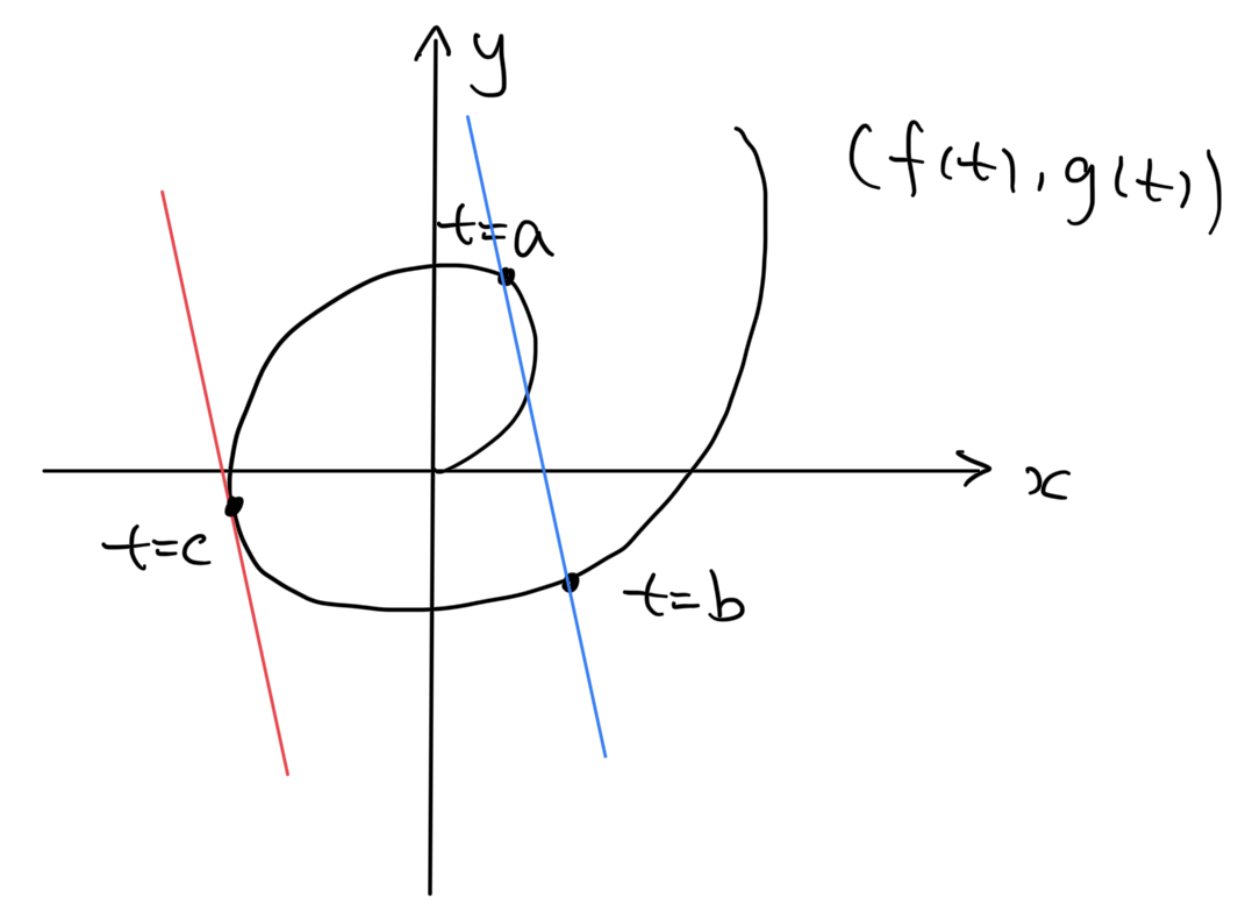
\includegraphics[scale=0.5]{fig/cauchy-mvt.png}
    \caption{Cauchy Mean Value Theorem}
    \label{fig:cauchy-mvt}
\end{figure}

The proof strategy is similar -- we aim to reduce this to \autoref{thm:rolle} (Rolle's Theorem).

\begin{proof}
    Let the function be
    \[
        \phi\pqty{x} = \bqty{g\pqty{x} - g\pqty{a}} \bqty{f\pqty{b} - f\pqty{a}} - \bqty{g\pqty{b} - g\pqty{a}} \bqty{f\pqty{x} - f\pqty{a}}.
    \]

    Note that
    \[
        \phi'\pqty{x} = g'\pqty{x} \pqty{f\pqty{b} - f\pqty{a}} - f'\pqty{x} \pqty{g\pqty{b} - g\pqty{a}},
    \]
    and we have
    \[
        \phi\pqty{a} = \phi\pqty{b} = 0.
    \]

    Applying \autoref{thm:rolle} (Rolle's Theorem) finishes the proof.
\end{proof}

\begin{theorem}[L'H\^{o}pital's Rule]
    \label{thm:l-hopitals}%
    Let \(\minusinfty \leq a < b \leq \plusinfty\). Let \(\functiondomain{f, g}{\oointv{a}{b}}{\RR}\) be differentiable, and \(g'\pqty{x} \neq 0\) for all \(x \in \oointv{a}{b}\). Suppose:
    \begin{itemize}
        \item the limit
        \[
            \lim_{x \to a} \frac{f'\pqty{x}}{g'\pqty{x}} = l
        \]
        exists, where \(l \in \RR \cup \Bqty{\pminfty}\) could be infinite;
        \item \(\lim_{x \to a} f\pqty{x} = \lim_{x \to a} g\pqty{x} = 0\); or \(\lim_{x \to a} g\pqty{x} = \pminfty\).
    \end{itemize}

    Then we have
    \[
        \lim_{x \to a} \frac{f\pqty{x}}{g\pqty{x}} = l.
    \]
\end{theorem}

\begin{proof}
    \textbf{\(\frac{0}{0}\) Case.} We may set \(f\pqty{a} = g\pqty{a} = 0\) in this case. We first note that \(g\pqty{x} \neq 0\). If so, then Rolle's theorem would imply that \(g'\pqty{t} = 0\) for some \(t\) between \(a\) and \(x\).

    By \autoref{thm:cauchy-mvt} (Cauchy's Mean Value Theorem), for any \(x \in \oointv{a}{b}\), there is some \(c\pqty{x} \in \oointv{a}{x}\), such that
    \[
        \frac{f'\pqty{c\pqty{x}}}{g'\pqty{c\pqty{x}}} = \frac{f\pqty{x} - f\pqty{a}}{g\pqty{x} - g\pqty{a}} = \frac{f\pqty{x}}{g\pqty{x}}.
    \]

    We have \(c\pqty{x} \to a\) as \(x \to a\), with \(c\pqty{x} \neq a\). Now, if we have
    \[
        \lim_{x \to a} \frac{f'\pqty{x}}{g'\pqty{x}} = l,
    \]
    then we have
    \[
        \lim_{x \to a} \frac{f'\pqty{c\pqty{x}}}{g'\pqty{c\pqty{x}}} = l,
    \]
    and hence
    \[
        \lim_{x \to a} \frac{f\pqty{x}}{g\pqty{x}} = l
    \]
    as desired.

    \textbf{\(\frac{?}{\infty}\) Case.} This case is mostly similar. We may first restrict the domain such that \(g\pqty{x} \neq 0\) anywhere. Let \(\epsilon > 0\) be arbitrary. Since \(\lim_{x \to a} \frac{f'\pqty{x}}{g'\pqty{x}} = l\), we have some \(\delta\pqty{\epsilon} > 0\), such that
    \[
        \forall x \in \oointv{a}{a + \delta}: \abs{\frac{f'\pqty{x}}{g'\pqty{x}} - l} < \epsilon.
    \]
    
    We fix \(d \in \oointv{a}{a + \delta}\) such that \(g\pqty{d}\) takes the same sign as \(\lim_{x \to a} g\pqty{x}\). For any \(x \in \oointv{a}{d}\), applying \autoref{thm:cauchy-mvt} (Cauchy's Mean Value Theorem), there is some \(c\pqty{x} \in \oointv{x}{d}\), such that
    \[
        \frac{f'\pqty{c\pqty{x}}}{g'\pqty{c\pqty{x}}} = \frac{f\pqty{x} - f\pqty{d}}{g\pqty{x} - g\pqty{d}}.
    \]

    Since \(c\pqty{x} \in \oointv{x}{d}\), we have \(c\pqty{x} \in \oointv{a}{a + \epsilon}\). Therefore, we have
    \[
        \abs{\frac{f\pqty{x} - f\pqty{d}}{g\pqty{x} - g\pqty{d}} - l} < \epsilon.
    \]

    Dividing top and bottom by \(g\pqty{x}\), we have
    \[
        \abs{\frac{\frac{f\pqty{x}}{g\pqty{x}} - \frac{f\pqty{d}}{g\pqty{x}}}{1 - \frac{g\pqty{d}}{g\pqty{x}}} - l} < \epsilon.
    \]

    This implies
    \[
        \abs{1 - \frac{g\pqty{d}}{g\pqty{x}}} \pqty{l - \epsilon} < \frac{f\pqty{x}}{g\pqty{x}} - \frac{f\pqty{d}}{g\pqty{x}} < \abs{1 - \frac{g\pqty{d}}{g\pqty{x}}} \pqty{l + \epsilon}.
    \]

    Therefore, taking \(x \to a\), we have
    \[
        l - \epsilon \leq \liminf_{x \to a} \frac{f\pqty{x}}{g\pqty{x}} \leq \limsup_{x \to a} \frac{f\pqty{x}}{g\pqty{x}} \leq l + \epsilon
    \]
    and taking \(\epsilon \to 0\) gives the desired result. (The final two lines could be replaced with more elementary \(\epsilon-\delta\)s, but I am just not bothered to do that.)
\end{proof}

\begin{example}[Application of L'H\^{o}pital's Rule]
    \label{ex:l-hopitals}%
    We have seen in \autoref{ex:sin-x-x-limit} that
    \[
        \lim_{x \to 0} \frac{\sin x}{x} = 1.
    \]

    L'H\^{o}pital's Rule tells us that
    \[
        \lim_{x \to 0} \frac{\sin x}{x} = \lim_{x \to 0} \frac{\cos x}{1} = 1.
    \]

    Behind the scenes in the rule, we have for some \(\theta \in \oointv{0}{1}\), that
    \[
        \frac{\sin x}{x} = \frac{\sin x - \sin 0}{x - 0} = \frac{\cos \pqty{\theta x}}{1}.
    \]
    
    Then we have
    \[
        \lim_{x \to 0} \frac{\sin x}{x} = \lim_{x \to 0} \cos \pqty{\theta x} = 1.
    \]
\end{example}

Similar to \autoref{ex:inverse-fn-differentiation}, we also have a statement about a \emph{local} function inverse.

\begin{proposition}[Local Inverse Function Theorem]
    \label{prop:local-ivt}%
    Let \(\functiondomain{f}{\ccintv{a}{b}}{\RR}\) be continuous on \(\ccintv{a}{b}\) and continuously differentiable on \(\oointv{a}{b}\). Suppose there is some \(x_0 \in \oointv{a}{b}\) such that \(f'\pqty{x_0} \neq 0\). Then there exists some \(\epsilon > 0\) with \(\ccintv{x_0 - \epsilon}{x_0 + \epsilon} \subseteq \oointv{a}{b}\) such that the restriction
    \[
        \functiondomain{f}{\oointv{x_0 - \epsilon}{x_0 + \epsilon}}{f\pqty{\oointv{x_0 - \epsilon}{x_0 + \epsilon}}}
    \]
    is bijective, and \(f\inverse\) is differentiable with derivative
    \[
        \pqty{f\inverse}'\pqty{y} = \frac{1}{f'\pqty{f\inverse\pqty{y}}}
    \]
    for all \(y \in f\pqty{\oointv{x_0 - \epsilon}{x_0 + \epsilon}}\).
\end{proposition}

\begin{proof}
    Since \(f\) is continuously differentiable, we have \(f'\) is continuous, so there is some neighbourhood about \(x_0\) in \(\oointv{a}{b}\), say \(\ccintv{x_0 - \epsilon}{x_0 + \epsilon}\), such that \(f'\pqty{x} > 0\) for all \(x\) in this interval. Then applying the \autoref{thm:inverse-fn-thm-differentiable} (Inverse Function Theorem for Differentiability) over this interval gives the result as desired.

    Concretely, to show such interval exist, we apply the definition of continuity on \(f'\) near \(x_0\). Take \(\epsilon = f'\pqty{x_0}\), then there is some \(\delta > 0\) such that
    \[
        \forall x \in \ccintv{a}{b}, \abs{x - x_0} < \delta: \abs{f'\pqty{x} - f'\pqty{x_0}} < f'\pqty{x_0}
    \]
    and hence, in particular,
    \[
        \forall x \in \ccintv{a}{b}, \abs{x - x_0} < \delta: f'\pqty{x} > 0.
    \]

    Now, note \(m = \min\Bqty{\delta, x_0 - a, b - x_0} > 0\), so take any \(0 < \epsilon < m\), then for all \(x \in \ccintv{x_0 - \epsilon}{x_0 + \epsilon}\), we have \(x_0 \in \ccintv{a}{b}\) and \(\abs{x - x_0} < \delta\), so \(f'\pqty{x} > 0\) for this restriction.
\end{proof}

\subsection{Darboux's Theorem}

A really cool application of \autoref{thm:extreme-value} (Extreme Value Theorem), \autoref{thm:mean-value-thm} (Mean Value Theorem) and \autoref{thm:intermediate-value} (Intermediate Value Theorem) is the following theorem.

\begin{theorem}[Darboux's Theorem]
    If \(\functiondomain{f}{\ccintv{a}{b}}{\RR}\) is differentiable with \(a < b\), then for all \(f'\pqty{a} < z < f'\pqty{b}\) or \(f'\pqty{b} < z < f'\pqty{a}\), there exists some \(c\) with \(a < c < b\), such that \(f'\pqty{c} = z\).
\end{theorem}

\begin{proof}[using \autoref{thm:extreme-value} (Extreme Value Theorem)]
    We assume that \(f'\pqty{a} < z < f'\pqty{b}\) and the other case is similar. We define the function \(\functiondomain{\phi}{\ccintv{a}{b}}{\RR}\) with
    \[
        \phi\pqty{x} = f\pqty{x} - zx.
    \]

    Since \(f\) is differentiable, it must be continuous, and by \autoref{thm:extreme-value} (Extreme Value Theorem), \(\phi\) attains its bounds.

    Let \(m \in \ccintv{a}{b}\) be such that
    \[
        \phi\pqty{m} = \inf_{x \in \ccintv{a}{b}} \phi\pqty{x}.
    \]

    First, if \(m = a\), then \(\phi\pqty{a} \leq \phi\pqty{x}\) for all \(x \in \ocintv{a}{b}\). Hence, we have
    \[
        f\pqty{a} - az \leq f\pqty{x} - xz.
    \]

    Rearranging, we have
    \[
        z \leq \frac{f\pqty{x} - f\pqty{a}}{x - a}
    \]
    and taking \(x \to a\) gives \(z \leq f'\pqty{a}\), which is a contradiction with \(z > f'\pqty{a}\). So \(m \neq a\)

    Similarly, \(m \neq b\), so \(m \in \oointv{a}{b}\).

    Hence, for any \(x \in \cointv{a}{m}\), we have \(\phi\pqty{x} \geq \phi\pqty{m}\) but \(x - m < 0\), so
    \[
        \frac{\phi\pqty{x} - \phi\pqty{m}}{x - m} \leq 0,
    \]
    and hence in the limit (the limit exists, since \(f\) is differentiable implies \(\phi\) is differentiable),
    \[
        \phi'\pqty{m} \leq 0.
    \]

    Similarly, considering \(x \in \ocintv{m}{b}\), we have \(\phi'\pqty{m} \geq 0\). So \(\phi'\pqty{m} = 0\), and hence \(f'\pqty{m} = z\), finishing our proof.
\end{proof}

\begin{proof}[using \autoref{thm:mean-value-thm} (Mean Value Theorem) and \autoref{thm:intermediate-value} (Intermediate Value Theorem)]
    We consider the helper functions
    \[
        g\pqty{x} = \begin{cases}
            f'\pqty{a}, & x = a, \\
            \frac{f\pqty{x} - f\pqty{a}}{x - a}, & a < x \leq b,
        \end{cases}
    \]
    and
    \[
        h\pqty{x} = \begin{cases}
            \frac{f\pqty{x} - f\pqty{b}}{x - b}, & a \leq x < b, \\
            f'\pqty{b}, & x = b.
        \end{cases}
    \]

    Now, note that
    \[
        g\pqty{b} = h\pqty{a} = \frac{f\pqty{a} - f\pqty{b}}{a - b}.
    \]

    Hence, for \(f'\pqty{a} < z < f'\pqty{b}\), it must lie within either the image of \(g\), or the image of \(h\), since \(g\) and \(h\) are both continuous, and by \autoref{thm:intermediate-value} (Intermediate Value Theorem). In the first case,
    \[
        z = \frac{f\pqty{t} - f\pqty{a}}{t - a}
    \]
    for some \(a < t \leq b\), and in the second case,
    \[
        z = \frac{f\pqty{t} - f\pqty{b}}{t - b}
    \]  
    for some \(a \leq t < b\). Either case, we have
    \[
        z = \frac{f\pqty{\alpha} - f\pqty{\beta}}{\alpha - \beta}
    \]
    for \(\ccintv{\alpha}{\beta} \subseteq \ccintv{a}{b}\).

    Therefore, by \autoref{thm:mean-value-thm} (Mean Value Theorem), we have
    \[
        z = f' \pqty{c}  
    \]
    for some \(\alpha < c < \beta\), and hence for some \(a < c < b\).
\end{proof}

\subsection{Higher Derivatives and Taylor's Theorem}
\begin{definition}[Higher Order Derivatives]
    \label{def:higher-order-derivatives}%
    Suppose \(\functiondomain{f}{X \subseteq \CC}{\CC}\) is differentiable on \(X\). We say the function \(f\) is \emph{twice differentiable} on \(X\), if
    \[
        \function{f'}{X}{\CC}{x}{f'\pqty{x}}
    \]
    is differentiable. We define \(f\) is \emph{\(k\)-times differentiable} similarly, and denote this as \(f \in \diffClass{k} \pqty{X}\).

    We say \(f\) is \emph{\(k\)-times continuously differentiable}, and denote this as \(f \in \contClass{k} \pqty{X}\), if \(f\) is \(k\)-times differentiable and the \(k\)-th derivative
    \[
        \function{f^{\pqty{k}}}{X}{\CC}{x}{f^{\pqty{k}}\pqty{x}}
    \]
    is continuous.
\end{definition}

Note that the function spaces (differentiability classes) have the following containment relationship.
\[
    \contClass{0}\pqty{X} \supset \diffClass{1}\pqty{X} \supset \contClass{1}\pqty{X} \supset \diffClass{2}\pqty{X} \supset \contClass{2}\pqty{X} \supset \cdots,
\]
and that note these are strict inclusions.

\begin{definition}[Smooth]
    \label{def:smooth}%
    We say \(\functiondomain{f}{X}{\CC}\) is \emph{smooth} if \(f \in \diffClass{k}\pqty{X}\) for all \(k \in \NN\), and we denote this as
    \[
        f \in \smoothClass \pqty{X}.
    \]
\end{definition}

We saw from \autoref{lem:linear-approximation-differentiability} that \(f\) differentiable at \(a\) means \(f\) can be well-approximated by a linear function near \(a\), by
\[
    f\pqty{x} \approx f\pqty{a} + f'\pqty{a} \pqty{x - a}.
\]

Similarly, we may have
\[
    f\pqty{x} \approx f\pqty{a} + f'\pqty{a} \pqty{x - a} + \frac{1}{2} f''\pqty{a} \pqty{x - a}^2
\]
and in fact if it is \(n\)-times differentiable, we have
\[
    f\pqty{x} \approx \sum_{k = 0}^{n} \frac{f^{\pqty{k}} \pqty{a}}{k!} \cdot \pqty{x - a}^{k}.
\]

We want to quantify how correct this approximation is -- i.e., we want to quantify the \emph{remainder}.

\begin{definition}[Taylor Polynomial, Taylor Series]
    \label{def:taylor-polynomial-series}%
    If \(\functiondomain{f}{X}{\CC}\) is \(n\)-times differentiable at \(x_0 \in X\), then for \(x_0 + h \in X\), the \emph{Taylor Polynomial} of degree \(n\) at \(x_0\) is defined as
    \[
        T_{n, f, x_0} \pqty{h} = \sum_{k = 0}^{n} \frac{f^{\pqty{k}} \pqty{x_0}}{k!} \cdot h^{k}.
    \]

    If \(f\) is smooth at \(x_0 \in X\), then the infinite series
    \[
        \sum_{k = 0}^{\infty} \frac{f^{\pqty{k}} \pqty{x_0}}{k!} \cdot h^{k}
    \]
    is the \emph{Taylor Series} of \(f\) at \(x_0\).
\end{definition}

We will see different versions of Taylor's Theorems, all of which aims to quantify what the remainder is, but giving it in different forms.

\begin{definition}[Taylor Remainder]
    Suppose \(\functiondomain{f}{X}{\CC}\) is \(\pqty{n - 1}\)-times differentiable at \(a \in X\). Then for \(h \in X\), we let
    \[
        R_{n, f, a} \pqty{h} = f\pqty{a + h} - T_{n - 1, f, a} \pqty{h} = f\pqty{a + h} - \sum_{k = 0}^{n - 1} \frac{f^{\pqty{k}} \pqty{a}}{k!} \cdot h^k
    \]
    be the \emph{Taylor remainder}.
\end{definition}

\subsubsection{Mean Value Forms of the Remainder}

\begin{theorem}[Taylor's Theorem with Lagrange Remainder]
    \label{thm:taylor-thm-langrange-remainder}%
    Let \(\functiondomain{f}{\ccintv{a}{a + h}}{\RR}\) be \(n\) times differentiable on \(\oointv{a}{a + h}\) and \(\pqty{n - 1}\) times continuously differentiable on \(\ccintv{a}{a + h}\). Then the \emph{Lagrange Form of the Remainder} gives the Taylor remainder in the form
    \[
        R_{n, f, a} \pqty{h} = \frac{h^n}{n!} \cdot f^{\pqty{n}} \pqty{a + \theta h},
    \]
    for some \(\theta \in \oointv{0}{1}\).
\end{theorem}

\begin{remarks}
    \begin{itemize}
        \item When \(n = 1\), this simply gives \autoref{thm:mean-value-thm} (Mean Value Theorem).
        \item Furthermore, there is nothing special about \(h > 0\): we could simply swap the bounds of the intervals (i.e. \(\ccintv{a}{a + h}\) to \(\ccintv{a + h}{a}\) and \(\oointv{a}{a + h}\) to \(\oointv{a + h}{a}\)), and we will still get a similar result.
        \item If \(f \in \contClass{n} \pqty{\oointv{c}{d}}\) with \(\ccintv{a}{a + h} \subset \oointv{c}{d}\), then note that \(f^{\pqty{n}}\) is continuous on the closed interval, hence bounded, and let
        \[
            M_n = \sup_{x \in \ccintv{a}{a + h}} \abs{f^{\pqty{n}} \pqty{x}}.
        \]

        Then
        \[
            \abs{R_{n, f, a} \pqty{h}} \leq M_n \cdot \frac{\abs{h}^n}{n!}
        \]
        and we have \(R_{n, f, a} \pqty{h} = \bigO \pqty{h^n}\) as \(h \to 0\), or in other words, the approximation gets better as the point \(a + h\) gets closer to \(a\). \textbf{However, this does not tell us that \(R_{n, f, a} \pqty{h} \to 0\) as \(n \to \infty\)}, or in other words, adding more terms does not necessarily make our approximation better. Even if \(f \in \smoothClass\), we still do not know how \(M_n\) behaves with \(n\). (In other words, there are smooth functions that are not analytic (on \(\RR\)).)
    \end{itemize}
\end{remarks}

\begin{proof}[(First Proof)]
    Without loss of generality, we let \(a = 0\). Let
    \[
        \function{\phi}{\ccintv{0}{h}}{\RR}{t}{f\pqty{t} - T_{n - 1, f, 0} \pqty{t} - \frac{t^n}{n!} \cdot B}
    \]
    where we pick the constant \(B\) such that \(\phi\pqty{h} = 0\). Note that \(\phi\) is continuous, and that its \(\pqty{n - 1}\)-th derivatives is continuous on \(\ccintv{0}{h}\) and its \(n\)-th derivatives exists on \(\oointv{0}{h}\). Note that \(\phi\pqty{0} = 0\) and also \(\phi^{\pqty{k}} \pqty{0} = 0\) for all \(k = 0, \ldots, n - 1\).

    Since we have
    \[
        \phi\pqty{0} = \phi\pqty{h} = 0,
    \] 
    by \autoref{thm:rolle} (Rolle's Theorem), we have some \(\theta_1 \in \oointv{0}{1}\) with \(\phi'\pqty{\theta_1 h} = 0\). Applying Rolle's Theorem again on the interval \(\ccintv{0}{\theta_1 h}\) with the function \(\phi'\), we have some \(\theta_2 \in \oointv{0}{1}\) with \(\phi''\pqty{\theta_2 \theta_1 h} = 0\).

    Hence, by induction, we have some \(\theta_1, \theta_2, \ldots, \theta_n \in \oointv{0}{1}\), such that
    \[
        \phi^{\pqty{n}} \pqty{\theta_n \theta_{n - 1} \cdots \theta_{2} \theta_{1} h} = 0.
    \]

    We set \(\theta = \theta_n \theta_{n - 1} \cdots \theta_{2} \theta_{1} \in \oointv{0}{1}\), and hence there exists some \(\theta \in \oointv{0}{1}\), such that
    \[
        f^{\pqty{n}} \pqty{t} - B = \phi^{\pqty{n}} \pqty{\theta h} = 0,
    \]
    and hence
    \[
        B = f^{\pqty{n}} \pqty{\theta h},
    \]
    is indeed an error term, as desired.
\end{proof}

The first proof almost certainly much easier than the proof below, but this proof generalises the remainder into a more general case, which would be introduced in \autoref{thm:taylor-thm-cauchy-remainder} (Cauchy Form) and \autoref{thm:taylor-thm-schlomilch-remainder} (Schl\"{o}milch Form).

\begin{proof}[(Second Proof)]
    Without loss of generality, set \(a = 0\). Let
    \[
        \function{g}{\ccintv{0}{h}}{\RR}{t}{f\pqty{h} - \sum_{k = 0}^{n - 1} \frac{f^{\pqty{k}} \pqty{t}}{k!} \cdot \pqty{h - t}^{k}.}
    \]

    Note that
    \[
        g\pqty{0} = f\pqty{h} - T_{n - 1, f, 0} \pqty{h}.
    \]  

    Note \(g\) is continuous on \(\ccintv{0}{h}\) and differentiable on \(\oointv{0}{h}\), with
    \[
        g'\pqty{t} = - \frac{f^{\pqty{n}}\pqty{t}}{\pqty{n - 1}!} \pqty{h - t}^{n - 1}.
    \]

    Therefore, for any \(p > 0\), set
    \[
        \phi_{p} \pqty{t} = g\pqty{t} - \frac{\pqty{h - t}^{p}}{h^p} g\pqty{0}.
    \]

    We may verify that \(\phi_{p} \pqty{h} = \phi_p \pqty{0} = 0\). Hence, by \autoref{thm:rolle} (Rolle's Theorem), there is some \(\theta \in \oointv{0}{1}\) such that
    \[
        \phi_p' \pqty{\theta h} = g' \pqty{\theta h} + \frac{p \pqty{h - \theta h}^{p - 1}}{h^p} \cdot g\pqty{0} = g'\pqty{\theta h} + \frac{p \pqty{1 - \theta}^{p - 1}}{h} \cdot g\pqty{0} = 0.
    \]

    Therefore, there is some \(\theta \in \oointv{0}{1}\), such that
    \[
        - \frac{h^{n - 1} \pqty{1 - \theta}^{n - 1}}{\pqty{n - 1}!} \cdot f^{\pqty{n}} \pqty{\theta h} + p \cdot \frac{\pqty{1 - \theta}^{p - 1}}{h} \cdot g\pqty{0} = 0.
    \]

    Hence, by rearranging, we have
    \[
        f\pqty{h} - T_{n - 1, f, 0} \pqty{h} = \frac{h^n}{p \pqty{n - 1}!} \pqty{1 - \theta}^{n - p} \cdot f^{\pqty{n}} \pqty{\theta h}.
    \]

    We take \(p = n\), and we have the result as desired.
\end{proof}

Although the second proof looks very horrible, this in fact gives another version of Taylor's theorem, with a different estimate -- since we can choose all \(p\)s!

\begin{theorem}[Taylor's Theorem with Cauchy Remainder]
    \label{thm:taylor-thm-cauchy-remainder}%
    Let \(\functiondomain{f}{\ccintv{a}{a + h}}{\RR}\) be \(n\) times differentiable on \(\oointv{a}{a + h}\) and \(\pqty{n - 1}\) times continuously differentiable on \(\ccintv{a}{a + h}\). Then the \emph{Cauchy Form of the Remainder} gives the Taylor remainder in the form
    \[
        R_{n, f, a} \pqty{h} = \frac{h^{n}}{\pqty{n - 1}!} \cdot \pqty{1 - \theta}^{n - 1} f^{\pqty{n}} \pqty{a + \theta h},
    \]
    for some \(\theta \in \oointv{0}{1}\).
\end{theorem}

\begin{proof}
    By putting \(p = 1\) into the second proof of \autoref{thm:taylor-thm-langrange-remainder}.
\end{proof}

\begin{remark}
    Similarly, if we have \(f \in \contClass{n} \pqty{\oointv{c}{d}}\) with \(\ccintv{a}{a + h} \subset \oointv{c}{d}\), then as in previous remark, we may set
    \[
        M_n = \sup_{x \in \ccintv{a}{a + h}} \abs{f^{\pqty{n}} \pqty{x}}
    \]
    and by \autoref{thm:taylor-thm-cauchy-remainder}, then we have
    \[
        \abs{R_{n, f, a} \pqty{h}} \leq M_n \cdot \frac{\abs{h}^n}{\pqty{n - 1}!}.
    \]
\end{remark}

This looks like an even worse estimate, since \(\pqty{n - 1}!\) on the denominator gives a bigger error than \(\pqty{n}!\). However, this is not necessarily true -- as the following example will demonstrate.

\begin{example}[Application of Taylor's Theorems]
    \label{ex:application-taylor}%
    Consider the function \(f\pqty{x} = x^q\) for some rational \(q \in \QQ\). This function is smooth on \(\oointv{0}{\plusinfty}\). We may attempt to calculate its derivates by
    \[
        f^{\pqty{k}} \pqty{x} = q \cdot \pqty{q - 1} \cdot \pqty{q - 2} \cdots \pqty{q - k + 1} \cdot x^{q - k}.
    \]

    We may calculate the Taylor polynomial at \(1\) as
    \[
        T_{n - 1, f, 1} \pqty{h} = \sum_{k = 0}^{n - 1} \frac{q \pqty{q - 1} \cdots \pqty{q - k + 1}}{k!} \cdot h^k = \sum_{k = 0}^{n - 1} \binom{q}{k} h^k.
    \]

    We now look at
    \[
        R_{n, f, 1} \pqty{h} = \pqty{1 + h}^{q} - \sum_{k = 0}^{n - 1} \binom{q}{k} h^k
    \]
    in \(\oointv{-1}{1}\). In particular, we would like to study if the remainder converges to \(0\) as \(n \to \infty\). (This is trivial for \(h = 0\).)

    We evaluate both remainders. If we use \autoref{thm:taylor-thm-langrange-remainder} (Lagrange Remainder), we have some \(\theta \in \oointv{0}{1}\) such that
    \[
        R_{n, f, 1} \pqty{h} = \binom{q}{n} \pqty{1 + \theta h}^{q - n} h^n.
    \]

    If \(n \geq q\), then \(\pqty{1 + \theta h}^{q - n} \leq 1\) for \(h \in \cointv{0}{1}\), and hence
    \[
        \abs{R_{n, f, 1} \pqty{h}} \leq \abs{\binom{q}{n} h^n} \to 0
    \]
    as \(n \to \infty\), for any \(h \in \cointv{0}{1}\). However, this argument fails for \(h \in \oointv{-1}{0}\).

    If we use \autoref{thm:taylor-thm-cauchy-remainder} (Cauchy Remainder), we have some \(\theta \in \oointv{0}{1}\) (not necessarily identical to the \(\theta\) before), that
    \begin{align*}
        R_{n, f, 1} \pqty{h} &= \binom{q}{n} \cdot n \cdot \pqty{1 - \theta}^{n - 1} \cdot \pqty{1 + \theta h}^{q - n} \cdot h^n \\
        &= \pqty{1 - \theta}^{n - 1} q \binom{q - 1}{n - 1} \pqty{1 + \theta h}^{q - n} h^n \\
        &= q \binom{q - 1}{n - 1} \cdot \pqty{\frac{1 - \theta}{1 + \theta h}}^{n - 1} \cdot \pqty{1 + \theta h}^{q - 1} h^n.
    \end{align*}

    Now, for any \(h \in \oointv{-1}{1}\), we have \(1 + \theta h = \pqty{1 - \theta} + \theta \pqty{h + 1} \geq 1 - \theta\). Hence, we have
    \[
        \pqty{\frac{1 - \theta}{1 + \theta h}}^{n - 1} \leq 1
    \]
    as long as \(n \geq 1\). Hence, we may apply a bound the remainder by
    \[
        \abs{R_{n, f, 1} \pqty{h}} \leq \abs{qh} \cdot \abs{\binom{q - 1}{n - 1} h^{n - 1}} \cdot \abs{1 + \theta h}^{q - 1}.
    \]

    Note that only the middle term depends on \(n\). Therefore,
    \[
        \abs{R_{n, f, 1} \pqty{h}} \to 0
    \]
    as \(n \to \infty\) for every \(h \in \oointv{-1}{1}\).
    
    So the Cauchy remainder gives us that the remainder is exponentially small as \(n \to \infty\), for all \(h \in \oointv{-1}{1}\), while the Lagrange remainder only guaranteed that for the range of \(h \in \cointv{0}{1}\).
\end{example}

\begin{definition}[Analytic Function]
    \label{def:analytic}%
    We say that \(f \in \smoothClass \pqty{\oointv{c}{d}}\) is \emph{analytic}, denoted as \(f \in \analyticClass \pqty{\oointv{c}{d}}\), if for every \(a \in \oointv{c}{d}\), there exists an \(r > 0\), such that for all \(\abs{h} < r\),
    \[
        f\pqty{a + h} = \sum_{k = 0}^{\infty} \frac{f^{\pqty{k}} \pqty{a}}{k!} \cdot h^k = \lim_{n \to \infty} T_{n, f, a} \pqty{h}.
    \]

    Equivalently, we have
    \[
        \lim_{n \to \infty} R_{n, f, a} \pqty{h} = 0.
    \]

    In other words, analytic functions are functions whose Taylor series at any point converges to the function within some non-zero radius.
\end{definition}

\begin{example}[Analytic Function]
    \label{ex:analytic-fn}%
    As in \autoref{ex:application-taylor}, the function \(x^q\) is analytic in \(\oointv{0}{2}\) -- in other words, \(\pqty{1 + x}^q\) is analytic in \(\oointv{-1}{1}\).
\end{example}

\begin{remark}
    Even if \(R_{n, f, a} \pqty{h} \notto 0\) as \(n \to \infty\), this \emph{does not mean} that the Taylor series
    \[
        \sum_{k = 0}^{\infty} \frac{f^{\pqty{k}} \pqty{a}}{k!} \cdot h^k
    \]
    does not converge -- it just means that the Taylor series does not converge to the actual function value. (In \(\RR\), there are smooth functions that are not analytic.)
\end{remark}

Finally, just for completeness, we introduce the name for the general form when we do not specify the value of \(p\).

\begin{theorem}[Taylor's Theorem with Schl\"{o}milch Remainder]
    \label{thm:taylor-thm-schlomilch-remainder}%
    Let \(\functiondomain{f}{\ccintv{a}{a + h}}{\RR}\) be \(n\) times differentiable on \(\oointv{a}{a + h}\) and \(\pqty{n - 1}\) times continuously differentiable on \(\ccintv{a}{a + h}\). Then the \emph{Schl\"{o}milch Form of the Remainder} gives the Taylor remainder in the form, for any fixed \(p > 0\),
    \[
        R_{n, f, a} \pqty{h} = \frac{h^{n}}{p \pqty{n - 1}!} \cdot \pqty{1 - \theta}^{n - p} f^{\pqty{n}} \pqty{a + \theta h},
    \]
    for some \(\theta \in \oointv{0}{1}\).
\end{theorem}

\begin{proof}
    Identical to the second proof of \autoref{thm:taylor-thm-langrange-remainder}.
\end{proof}

\subsubsection{Asymptotic Form of the Remainder}

This section is not mentioned in the lecture, but I think it just really makes sense to include it here.

A good question to ask is, must the Taylor polynomial be correct up to its degree? Is there a better degree-\(n\) polynomial that fits the function better?

\begin{theorem}[Taylor's Theorem with Peano Remainder]
    \label{thm:taylor-thm-peano-remainder}%
    Let \(\functiondomain{f}{\oointv{c}{d}}{\RR}\) be \(\pqty{n - 1}\) times differentiable. Then for any \(a \in \oointv{c}{d}\), the \emph{Peano Form of the Remainder} gives the Taylor remainder in the form
    \[
        R_{n, f, a} \pqty{h} = \littleO\pqty{h^{n - 1}}.
    \]
\end{theorem}

\begin{proof}
    We may show this by induction on \(n\), and using \autoref{thm:l-hopitals} (L'H\^{o}pital's Rule). Without loss of generality, let \(a = 0\). Recall from the definition of the little-\(\littleO\) notation, that we want to show
    \[
        \lim_{h \to 0} \frac{R_{n, f, 0} \pqty{h}}{h^{n - 1}} = 0.
    \]

    The base case where \(n = 1\) is trivial, and for \(n = 2\) is proven in \autoref{lem:linear-approximation-differentiability}.

    For the general case, recall that
    \[
        R_{n, f, 0} \pqty{h} = f\pqty{h} - \sum_{k = 0}^{n - 1} \frac{f^{\pqty{k}} \pqty{0}}{k!} \cdot h^k.
    \]

    Since \(f\) is \(\pqty{n - 1}\) times differentiable at \(0\), we have \(R\) is \(\pqty{n - 1}\) times differentiable at \(0\), and in particular, continuous. Hence,
    \[
        \lim_{h \to 0} R_{n, f, 0} \pqty{h} = R_{n, f, 0} \pqty{0} = 0.
    \]
    
    Therefore, this satisfies the setup of L'H\^{o}pital's Rule, and hence we calculate the derivative of \(R_{n, f, a} \pqty{h}\). We note
    \[
        R'_{n, f, 0} \pqty{h} = f'\pqty{h} - \sum_{k = 1}^{n - 1} \frac{f^{\pqty{k}} \pqty{0}}{\pqty{k - 1}!} \cdot h^{k - 1} = f'\pqty{h} - \sum_{k = 0}^{n - 2} \frac{f^{\pqty{k + 1}} \pqty{0}}{k!} \cdot h^k = R_{n - 1, f', 0} \pqty{h}.
    \]

    Therefore, it suffices to show for \(f'\) (which is \(\pqty{n - 2}\) times differentiable), that
    \[
        R_{n - 1, f', 0} \pqty{h} = \littleO\pqty{h^{n - 2}}.
    \]

    This is indeed true by our induction hypothesis.
\end{proof}

This result shows that the remainder term must have strictly higher order than \(h^{n - 1}\), and hence Taylor's Polynomial is indeed the best \(n\)-th order polynomial we can get, in the asymptotic sense.